\documentclass[pdf, aspectratio=169]{beamer}
\usepackage[]{hyperref,graphicx,siunitx,lmodern,booktabs,tikz,wasysym,caption}
\usepackage{pdfpc-commands}
\usepackage[mode=buildnew]{standalone}
\mode<presentation>{\usetheme{Astro}}

\makeatletter
\let\@@magyar@captionfix\relax
\makeatother

\sisetup{per-mode=symbol}
\usetikzlibrary{calc,angles,quotes}
\graphicspath{ {../Images/} }

%preamble
\title{Luke! Use the Force!}
\date{September 10, 2018}
\author{Jed Rembold}

\begin{document}
\renewcommand*{\theenumi}{\Alph{enumi}}

\begin{frame}{Announcements}
	\begin{itemize}
		\item New WebWorK due Wednesday!
		\item Lab tonight for Group B!
		  \begin{itemize}
		    \item Already posted for you to print on the website
			\item Meet in Collins 324
		  \end{itemize}
		\item Poll: \url{rembold-class.ddns.net}
	\end{itemize}
\end{frame}

\begin{frame}{APOD!}
	\begin{center}
		\href{https://apod.nasa.gov/apod/ap180831.html}{\includegraphics[width=.6\textwidth]{APOD_Mars.jpg}}
	\end{center}
\end{frame}

\begin{frame}{Review Question}
	Halley's comet has a period of 76 years. At it's closest approach, it is about 0.6 AU from the Sun. What is the maximum distance Halley's comet reaches from the Sun? (\emph{Hint: You can ``undo'' a cubed by taking the cube root or raising it to the 1/3 power})
	\begin{enumerate}
		\item \SI{17.94}{AU}
		\item \alert<2>{\SI{35.28}{AU}}
		\item \SI{35.88}{AU}
		\item \SI{75.4}{AU}
	\end{enumerate}
	
  
\end{frame}

\begin{frame}[t]{Enter Galileo!}
  \begin{columns}[t]
	\column{.45\textwidth}
	\begin{block}{Kepler}
	  \begin{itemize}
		\item Derived entirely from Brahe's naked eye observations
		\item Only ``proof'' was that they explain everything nice and simple
	  \end{itemize}
	\end{block}
	\column{.45\textwidth}
	\begin{block}{Galileo}
	  \begin{itemize}
		\item Strongly believed in Copernicus's heliocentric solar system
		\item Wanted to \emph{prove} that the Earth orbited the Sun
		\item Did not \emph{invent} the telescope, but was almong the first to use it to study the heavens
		\item Widely published his findings
	  \end{itemize}
	\end{block}
  \end{columns}
\end{frame}

\begin{frame}{The Observations of Galileo}
  \begin{center}
	\begin{tikzpicture}
	  \begin{scope}
		\clip (0,0) rectangle (5,7);
		\node[anchor=south west] at (0,0) {\includegraphics[width=10cm]{ch4_gal_moons.jpg}};
	  \end{scope}
	  \node[anchor=south west] at (5,2.5) {\includegraphics[width=4.3cm]{ch4_gal_moon.png}};
	  \node[anchor=south west] at (5,0) {\includegraphics[width=5cm]{ch4_gal_phases.jpg}};
	\end{tikzpicture}
  \end{center}
\end{frame}

\begin{frame}{Sunspots!}
  \begin{figure}[h!]
	\centering
	\includegraphics[width=.7\textwidth, height=.5\textwidth, keepaspectratio]{ch4_gal_sunspots.png}
  \end{figure}
\end{frame}

\begin{frame}{More Modern Phases of Venus}
  \begin{figure}[h!]
	\centering
	\includegraphics[width=\textwidth]{ch4_venus_phase.jpg}
  \end{figure}
\end{frame}

\begin{frame}{The Physics of Galileo!}
  \begin{columns}
	\column{.5\textwidth}
	\begin{itemize}
	  \item Disputed ``classical'' Aristotle physics
	  \item Made large strides in how we think about:
		\begin{itemize}
		  \item<2-> Relative Motion
		  \item<3-> Inertia
		  \item<4-> Falling bodies
		  \item<5-> Projectiles
		\end{itemize}
	\end{itemize}
	\column{.5\textwidth}
	\begin{figure}[h!]
	  \centering
	  \includegraphics<4>[width=.8\textwidth, height=.8\textwidth, keepaspectratio]{ch4_pisa.jpg}
	  \includegraphics<5>[width=\textwidth]{ch4_gal_projectile.png}
	  \includegraphics<2>[width=\textwidth]{ch4_gal_relmot.jpg}
	  \includegraphics<3>[width=\textwidth]{ch4_gal_incline.jpg}
	\end{figure}
  \end{columns}
\end{frame}

\begin{frame}{Kepler and Galileo}
  \begin{columns}
	\column{.5\textwidth}
	\begin{itemize}
	  \item Around during the same time period
		\begin{itemize}
		  \item Keplers first Laws published in 1609
		  \item Galileo's first telescope observations 1610
		\end{itemize}
	  \item Despite church resistance, the heliocentric model gain acceptance over the next 50 years
	\end{itemize}
	\column{.5\textwidth}
	\begin{center}
	  \begin{tikzpicture}
		\onslide<1>{
		  \node (img) at (0,0) {\includegraphics[width=.5\textwidth]{ch4_kepler.jpg}};
		  \node[below] at (img.south) {Kepler: 1571-1630};
		}
		\onslide<2>{
		  \node (img) at (0,0) {\includegraphics[width=.5\textwidth]{ch4_galileo.jpg}};
		  \node[below] at (img.south) {Galileo: 1564-1642};
		}
	  \end{tikzpicture}
	\end{center}
  \end{columns}
\end{frame}
\begin{frame}{Good Sir Isaac}
  \begin{columns}
	\column{.5\textwidth}
	\begin{figure}[h!]
	  \centering
	  \includegraphics[width=.6\textwidth]{ch4_isaac.jpg}
	  \caption*{Isaac Newton: 1642-1727}
	\end{figure}
	\column{.5\textwidth}
	\begin{itemize}
	  \item Was able to relate the behavior of orbiting bodies to the behavior of bodies on Earth
	  \item Short and Succinct: Summarized everything in four sentences\ldots
	\end{itemize}
  \end{columns}
\end{frame}

\begin{frame}{Newton's First Law}
  \begin{alertblock}{Newton's First Law}
	A body continues in a state of rest or uniform motion in a straight line unless acted on by a force.
  \end{alertblock}
  \begin{itemize}
	\item Implications for astronomy?
	  \begin{itemize}
		\item A object that falls when released must be feeling a force
		\item An object moving in a circle must have a force acting upon it, else it would travel in a straight line
	  \end{itemize}
	\item Generally thought of as the inertia law
  \end{itemize}
\end{frame}

\begin{frame}{Newton's Second Law}
  \begin{alertblock}{Newton's Second Law}
	The force on an object is equal to the mass of the object multiplied by its acceleration.
	\[\scalebox{4}{F = ma}\]
  \end{alertblock}
  \begin{itemize}
	\item An acceleration is analogous to a change in motion
	\item Such a change in motion depends only on the force applied and the mass of the object
	\item \alert{The change in motion is in the same direction as the force!}
  \end{itemize}
\end{frame}

\begin{frame}{Force Examples}
  \begin{columns}
	\column{.5\textwidth}
	\begin{figure}[h!]
	  \centering
	  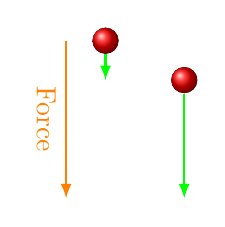
\begin{tikzpicture}
		\node[fill, ball color=red, circle] (ball1) at (0,0) {};
		\draw[thick, green, -latex] (ball1) --+(0,-0.5);
		\node[fill, ball color=red, circle] (ball2) at (1,-.5) {};
		\draw[thick, green, -latex] (ball2) --+(0,-1.5);
		\draw[thick, orange, -latex] (-0.5,0) -- node[midway,sloped,below] {Force} (-0.5, -2);
	  \end{tikzpicture}
	  \caption*{A ball dropping must feel a force to accelerate downwards!}
	\end{figure}
	\column{.5\textwidth}
	\begin{figure}[h!]
	  \centering
	  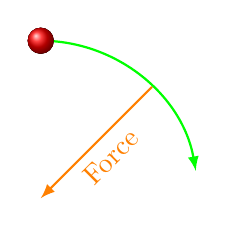
\begin{tikzpicture}
		\node[fill, ball color=red, circle] (ball1) at (0,2) {};
		\draw[thick, green, -latex] (ball1) arc (90:10:2cm);
		\node[fill, ball color=red, circle] (ball1) at (0,2) {};
		\draw[thick, orange, -latex] (45:2cm) -- node[midway,sloped,below] {Force} (0,0);
	  \end{tikzpicture}
	  \caption*{A ball curving at a constant speed must still feel a force turning it!}
	\end{figure}
  \end{columns}
\end{frame}

\begin{frame}{Basic Units}
  \begin{itemize}
	\item To compare our equations and answers, we really need a standard way of measuring things.
	\item In science (or if you live anywhere besides the US or England) this is the SI metric system
	  \begin{itemize}
		\item \alert{Meters} for distance
		\item \alert{Seconds} for time
		\item \alert{Kilograms} for mass
	  \end{itemize}
	\item All other SI units are defined in terms of these base units
	  \[\SI{1}{\newton} = \SI{1}{\kilo\gram\meter\per\second^2}\]
	\item For most physics formula:
	  \begin{itemize}
		\item SI Units \textcolor{green}{In} = SI Units \textcolor{red}{Out}
		\item Non-SI Units \textcolor{green}{In} = \underline{IT IS A MYSTERY} \textcolor{red}{Out}
	  \end{itemize}
  \end{itemize}
\end{frame}

\begin{frame}{The Standards}
  \vspace{-6mm}
  \begin{columns}[t]
	\column{.33\textwidth}
	\begin{block}{Meters}
	  \begin{itemize}
		\item Originated in France
		\item 1/10 millionth of the equator to North Pole distance
		\item Now defined officially by the wavelength of the orange-red light of burning Krypton
	  \end{itemize}
	\end{block}
	\column{.33\textwidth}
	\begin{block}{Second}
	  \begin{itemize}
		\item Defined as 1/86400 of a solar day
		\item Irregularies in Earth's rotation made this tricky
		\item Now defined in terms of atomic vibrations in Cesium atoms
	  \end{itemize}
	\end{block}
	\column{.33\textwidth}
	\begin{block}{Kilogram}
	  \begin{itemize}
		\item The mass of this cylindrical block of metal:
	  \end{itemize}
	  \begin{center}
		\includegraphics[width=.7\textwidth]{ch4_kilogram.jpg}
	  \end{center}
	\end{block}
  \end{columns}
\end{frame}

\begin{frame}{The Newton}
  \begin{itemize}
	\item The SI unit for force is the \alert{Newton} (\si{\newton})
	  \begin{itemize}
		\item A \SI{1}{\newton} force accelerates a \SI{1}{\kilo\gram} mass by \SI{1}{\meter\per\second} each second
	  \end{itemize}
  \end{itemize}
  \begin{center}
	\begin{tikzpicture}
	  \node[thick,draw=Blue,fill=Blue2, minimum width=1cm, minimum height=1cm] (block) at (0,0) {\SI{1}{\kilo\gram}};
	  \draw[orange,thick,latex-] (block.west) -- node[above] {\SI{1}{\newton}} +(-1,0);
	  \draw[green, thick, -latex] (block.east) -- node[above right] {\SI{0}{\meter\per\second}} + (0.2,0);
	  \node[thick,draw=Blue,fill=Blue2, minimum width=1cm, minimum height=1cm] (block2) at (1,-1.5) {\SI{1}{\kilo\gram}};
	  \draw[orange,thick,latex-] (block2.west) -- node[above] {\SI{1}{\newton}} +(-1,0);
	  \draw[green, thick, -latex] (block2.east) -- node[above right] {\SI{1}{\meter\per\second}} + (1,0);
	  \node[thick,draw=Blue,fill=Blue2, minimum width=1cm, minimum height=1cm] (block3) at (3,-3) {\SI{1}{\kilo\gram}};
	  \draw[orange,thick,latex-] (block3.west) -- node[above] {\SI{1}{\newton}} +(-1,0);
	  \draw[green, thick, -latex] (block3.east) -- node[above right] {\SI{2}{\meter\per\second}} + (2,0);
	\end{tikzpicture}
  \end{center}
\end{frame}



\begin{frame}{Circular Motion}
  \begin{itemize}
	\item Of particular interest to us is circular motion, since such motion largely describes the motion of the planets
	\item Newton tells us that, even if our planets are moving at a constant speed, a force \alert{must} be present to keep them moving in a circular orbit
	  \begin{center}
		\begin{tikzpicture}[scale=0.7]
		  \fill[inner color=yellow, outer color=orange] (0,0) circle (1cm);
		  \draw[dashed, -latex, thick] (3,0) arc (0:340:3cm);
		  \onslide<2->{
			\foreach \a in {0,45,...,350}{
			  \draw[orange, -latex] (\a:2.7) -- (\a:1.3);
			}
		  }
		  \node at (3,0) {\includegraphics[width=1cm]{world.png}};
		  \onslide<3>{\node[fill=Blue2, rounded corners, text=fg, align=center, anchor=west] at (4,-2) {But what is this\\regulating force?};}
		\end{tikzpicture}
	  \end{center}
  \end{itemize}
\end{frame}

\begin{frame}{Sup G?}
  \begin{itemize}
	\item Gravity! The universal attractor
	  \begin{itemize}
		\item Anything with mass attracts anything else with mass
		\item Strength of force depends on the masses involved
		\item Strength of the force diminished rapidly with distance
	  \end{itemize}
  \end{itemize}
  \begin{center}
	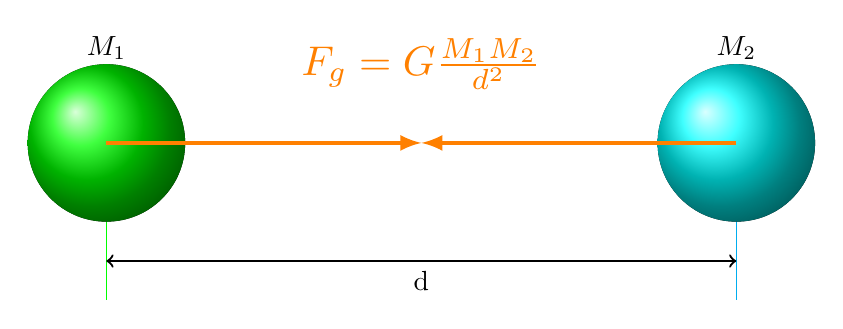
\begin{tikzpicture}
	  \coordinate (ball1) at (0,0);
	  \coordinate (ball2) at (8,0);
	  \coordinate (d) at ($(ball1)-(0,1.5)$);
	  \draw[green] (ball1) --+(0,-2);
	  \draw[cyan] (ball2) --+(0,-2);
	  \fill[ball color=green] (ball1) circle (1cm);
	  \fill[ball color=cyan] (ball2) circle (1cm);
	  \node at ($(ball1)+(0,1.2)$) {$M_1$};
	  \node at ($(ball2)+(0,1.2)$) {$M_2$};
	  \draw[<->, thick] (d) -- node[midway,below] {d} (d-|ball2);
	  \draw[-latex, ultra thick,orange] (ball1) -- +(4,0);
	  \draw[-latex, ultra thick,orange] (ball2) -- +(-4,0);
	  \node[orange] at (4,1) {\scalebox{1.5}{$F_g = G \frac{M_1 M_2}{d^2}$}};
	\end{tikzpicture}
  \end{center}
\end{frame}

\begin{frame}{The Gravitational Constant G}
  \begin{itemize}
	\item What is the gravitational force between:
	  \begin{itemize}
		\item Two \SI{1}{\kilo\gram} masses (say pineapples)
		\item 1 meter apart?
	  \end{itemize}
	  \begin{center}
		\begin{tikzpicture}
		  \node at (0,0) {\includegraphics[width=1cm]{ch4_pineapple.png}};
		  \node at (5,0) {\includegraphics[width=1cm]{ch4_pineapple.png}};
		  \draw[latex-latex, ultra thick] (0,-.4) -- node[above] {\SI{1}{\meter}} (5,-.4);
		  \onslide<2->{\node[orange] at (2.5,-1) {About \SI{6.7E-11}{\newton}};}
		\end{tikzpicture}
	  \end{center}
	\item<3> $G$ indicates the scale of the gravitational force in your units
	\item<3> $G=\SI{6.67E-11}{\newton\meter^2\per\kilo\gram^2}$
	\item<3> You must be using standard units to match $G$!
  \end{itemize}
\end{frame}

\begin{frame}{Gravitational Force on You!}
  \begin{example}
	Let's find the force of gravity between you, an average \SI{70}{\kilo\gram} individual, and the Earth, with its \SI{5.97E24}{\kilo\gram} mass. The Earth has an average radius of \SI{6378}{\kilo\meter}. What acceleration do you experience?
	\onslide<2->{
	  \[F_g = (\SI{6.67E-11}{})\frac{(\SI{5.97E24}{})(70)}{(6378000)^2} = \SI{685.2}{\newton}\]
	}
	\onslide<3->{
	  \[F_g = ma = \SI{685.2}{\newton} = (70)a \quad\Rightarrow a = \SI{9.79}{\meter\per\second^2}\]
	}
  \end{example}
\end{frame}

%\begin{frame}{The Fine Art of Throwing Things}
  %\begin{itemize}
	%\item Say you throw a ball sideways
	  %\begin{itemize}
		%\item<2-> You force the ball (using your arm) up to some speed
		%\item<3-> Inertia keeps the ball moving forward at that speed
		%\item<4-> Gravity drags the ball down
	  %\end{itemize}
  %\end{itemize}
  %\begin{center}
	%\begin{tikzpicture}
	  %\node at (0,0) {\includegraphics[width=3cm]{ch4_thrower.pdf}};
	  %%\fill[ball color=orange] (0,0) circle (3pt);
	  %\onslide<1>{\fill[ball color=green] (115:1.5) coordinate (p1) circle (3pt);}
	  %\onslide<2>{
		  %\fill[ball color=green] ($(p1)+(1,0)$) coordinate (p2) circle (3pt);
		%\draw[orange, thick,-latex] (p1) -- +(.9,0);
	  %}
	  %\onslide<3>{
		%\fill[ball color=green] ($(p2)+(1,0)$) circle (3pt);
	  %}
	  %\onslide<4>{
		%\foreach[count=\x] \y in {1.8,1.5, 0.9, 0.2, -.6, -1.5}{
		  %%\fill[ball color=green, opacity=\x/6] (2+\x,\y) circle (3pt);
		  %\fill[ball color=green, opacity=\x/6] ($(p2)+(\x+1,{\y-1.8})$) circle (3pt);
		%}
	  %}
	%\end{tikzpicture}
  %\end{center}
%\end{frame}

%\begin{frame}{One Powerful Arm\ldots}
  %\begin{itemize}
	%\item Now, if we hiked up a tall mountain and had a REALLY REALLY strong arm\ldots
	%\item \href{http://galileoandeinstein.physics.virginia.edu/more_stuff/flashlets/NewtMtn/home.html}{Newton's Mountain}
  %\end{itemize}
%\end{frame}

%%\begin{frame}{Review Question}
  %%Current events question! Tonight is:
  %%\begin{enumerate}
	%%\item The first full moon of the month
	%%\item The second full moon of the month (called the Blue Moon)
	%%\item \alert<2>{The first quarter moon of the month}
	%%\item The first new moon of the month
  %%\end{enumerate}
%%\end{frame}

%\begin{frame}{Moon Orbits}
  %\begin{itemize}
	%\item So we know that we can get an object into orbit by throwing it really hard in a certain direction
	%\item Whatever process formed the Moon must have thus given it this ``initial velocity''
	%\item So our Moon's orbit is a result of:
	  %\begin{itemize}
		%\item That velocity
		%\item Inertia
		%\item and the pull of gravity
	  %\end{itemize}
  %\end{itemize}
  %\begin{flushright}
	%\vspace{-2cm}
	%\begin{tikzpicture}
	  %\node at (0,0) {\includegraphics[width=1cm]{world.png}};
	  %\draw[dashed, help lines] (0,0) circle (2cm);
	  %\coordinate (moon) at (135:2cm);
	  %\draw[-latex, green, thick] (moon) -- node[midway,sloped,above] {\scriptsize Inertia} +(225:1cm);
	  %\fill[ball color=black!20] (moon) circle(1mm);
	  %\foreach \a in {45,90,...,360}{
		%\draw[-latex, orange, thick] (\a:1.8) -- (\a:1.1);
	  %}
	  %\node[align=center,orange, font=\scriptsize] at (2,-2) {Gravity pulls\\Moon toward\\Earth};
	%\end{tikzpicture}
  %\end{flushright}
%\end{frame}


%%\begin{frame}{Cavendish Experiment}
  %%\begin{itemize}
	%%\item A method to measure a tiny amount of gravitational force to determine $G$
  %%\end{itemize}
  %%\begin{center}
	%%\begin{tikzpicture}
	  %%\onslide<1>{
		%%\draw[LOrange, line width=3pt] (2,0) -- (-2,0);
		%%\fill[ball color=LOrange] (2,0) circle (2mm);
		%%\fill[ball color=LOrange] (-2,0) circle (2mm);
		%%\draw[Blue,line width=4pt] (0,2) -- (0,-2);
		%%\fill[ball color=Blue] (0,2) circle (5mm);
		%%\fill[ball color=Blue] (0,-2) circle (5mm);
		%%\draw[line width=4pt] (4pt,2mm) -- (4pt,-2mm);
		%%\draw[red,thick] (6pt,0) --+(-20:3cm);
	  %%}
	  %%\onslide<2>{
		%%\begin{scope}[rotate=60]
		  %%\draw[LOrange, line width=3pt] (2,0) -- (-2,0);
		  %%\fill[ball color=LOrange] (2,0) circle (2mm);
		  %%\fill[ball color=LOrange] (-2,0) circle (2mm);
		%%\end{scope}
		%%\begin{scope}[rotate=-5]
		  %%\draw[Blue,line width=4pt] (0,2) -- (0,-2);
		  %%\fill[ball color=Blue] (0,2) circle (5mm);
		  %%\fill[ball color=Blue] (0,-2) circle (5mm);
		  %%\draw[line width=4pt] (4pt,2mm) -- (4pt,-2mm);
		%%\end{scope}
		%%\draw[dashed,red!30,thick] (6pt,0) --+(-20:3cm);
		%%\draw[red,thick] (6pt,0) --+(-25:3cm) node[xshift=5mm,right,fg,align=left, font=\scriptsize] {Movement and\\oscillations\\used to determine\\gravitational constant};
	  %%}
	  %%\draw[rotate=19, fill=black!20, rounded corners] (2.7cm,-2mm) rectangle (4.0cm,2mm);
	  %%\draw[red,thick] (6pt,0) --+(20:2.5cm);
	%%\end{tikzpicture}
  %%\end{center}
%%\end{frame}

%\begin{frame}{Newton meets Kepler's 3rd}
  %\begin{itemize}
	%\item Recall that Kepler had worked out that
	  %\[\frac{a^3}{p^2}= \text{ same value for all planets orbiting Sun}\]
	  %\begin{itemize}
		%\item \alert{This is why we need to use AU and year units, because those describe Earth's $a$ and $p$!}
	  %\end{itemize}
	%\item<2> Newton worked out from theory that two objects held in orbit by gravity would obey:
	  %\[\frac{a^3}{p^2} = \frac{G \left( M_1 + M_2 \right)}{4\pi^2}\]
	  %where
	  %\vspace{-2mm}
	  %\scriptsize
	  %\begin{align*}
		%M_1, M_2 &= \text{ masses of objects in \underline{kilograms}}\\
		%a &= \text{ average separation of objects in \underline{meters}}\\
		%p &= \text{ orbital period in \underline{seconds}}\\
		%G &= \text{ gravitational constant in \underline{SI Units}}
	  %\end{align*}
  %\end{itemize}
%\end{frame}

%\begin{frame}{A Nicer Newton's Formulation}
  %\begin{itemize}
	%\item Put into more everyday units, Newton's formulation boils down to:
		%\[\frac{a^3}{p^2} = (M_1 + M_2)\]
	  %where
	  %\vspace{-2mm}
	  %\begin{align*}
		  %M_1, M_2 &= \text{ masses of objects in \alert{solar masses}}\\
		%a &= \text{ average separation of objects in \alert{AU}}\\
		%p &= \text{ orbital period in \alert{years}}\\
	  %\end{align*}
  %\item For the Sun and Earth, $M_1 + M_2 \approx 1$
  %\end{itemize}
%\end{frame}

%\begin{frame}{Newton and Kepler's 3rd Law Example}
  %\begin{example}
	%Suppose our Sun suddenly grew to have 30 times it's current mass. Assuming we stayed the same distance away, how long would our new year be?
	%\begin{itemize}
	  %\item $a = \SI{149.6E9}{\meter}$
	  %\item $M_{earth} = \SI{5.972E24}{\kilo\gram}$
	  %\item $M_{sun} = \SI{2.0E30}{\kilo\gram}$
	%\end{itemize}
	%\onslide<2>{
	  %\begin{align*}
		%p &= \sqrt{\frac{a^3}{\left( M_e + 30M_s \right)}}\\
		%&= \SI{0.18257}{yrs}\\
		%&= \SI{66.5}{days}
	  %\end{align*}
	%}
  %\end{example}
%\end{frame}

%\begin{frame}{Angular Momentum}
  %\begin{itemize}
	%\item Basically analogous to normal momentum but for things moving in circles
	%\item For an object moving in a circle, the \alert{angular momentum} is:
	  %\[L = m\times v \times r\]
	%\item The only way to change an objects angular momentum is to apply an angular force (called a torque)
  %\end{itemize}
  %\begin{center}
	%\begin{tikzpicture}
	  %\draw[help lines, dashed] (0,0) circle (2cm);
	  %\node[draw, circle, orange, fill=LOrange, text=black] (m) at (45:2) {$m$};
	  %\draw[thick] (0,0) -- node[midway, fill=Background] {$r$} (m);
	  %\draw[very thick, cyan, -latex] (m) --+(-45:1) node[below] {$v$};
	%\end{tikzpicture}
  %\end{center}
%\end{frame}

%\begin{frame}{Figure Skating}
	%\begin{center}
	  %\inlineMovie{../Videos/SkaterSpin.ogv}{../Videos/SkaterSpin.jpg}{width=.8\textwidth}
	%\end{center}
%\end{frame}

\end{document}
